\part{Caracterización de Amplificadores Operacionales}

\section{Construcción del circuito}

Uno de los objetivos de este trabajo fue analizar las características de los amplificadores operacionales (\textit{opamps}) y contrastarlos. En este caso, se los analizó en el contexto de un circuito amplificador no inversor (Figura \ref{fig:e2_ninv}).

\begin{figure}[ht]
	\begin{center}
		\begin{circuitikz}[american voltages]
		\draw
		(6,7) node[op amp, noinv input up] (opamp) {}
		(opamp.+) to [R, l_=$R_3$] ++(-2,0) to [sinusoidal voltage source=$V_{in}$] ++(0,-5) node [ground] {}
		(opamp.out) to (9,7) node[right] {$v_{out}$}
		(opamp.-) to ++(0,-2) coordinate(tmp)
		(tmp) to[R=$R_1$,*-] ++(0,-2) node[ground] {}
		(tmp) to[R=$R_2$] ++(3,0) to [short,-*] ++(0,2.5)
		;
	\end{circuitikz}
	\caption{Circuito Amplificador No Inversor}
	\label{fig:e2_ninv}
	\end{center}
\end{figure}

Los valores de las resistencias fueron los mostrados en el Cuadro \ref{tab:e2_res_val} 

\begin{table}[ht]
\begin{center}
\begin{tabular}{||c|c|c|c||}
	\hline
	Componente	&	Valor por Consigna	&	Valor Comercial ($\pm 5 \%)$)	& Valor Medido \\
	\hline
	$R_1$	&	$4 k\Omega$	&	$3.9 k\Omega$	&	$3.89 k\Omega$\\	
	$R_2$	&	$320 k\Omega$	&	$330 k\Omega$	&	$325 k\Omega $\\
	$R_3$	&	$220 k\Omega$	&	$220 k\Omega$	&	$212.3 k\Omega$\\
	\hline
\end{tabular}

\end{center}
\caption{Valores de las Resistencias}
\label{tab:e2_res_val}
\end{table}

Los \textit{opamps} utilizados fueron el $LM833N$ y el $NE5534P$, ambos alimentados con $\pm15 VCC$. Los circuitos fueron construidos sobre una \textit{protoboard}.

\subsection{Caso Ideal}
En un modelo teórico ideal el \textit{opamp} tendría una impedancia de entrada con magnitud infinita, y por lo tanto no fluiría corriente a travéz de las terminales del \textit{opamp}, lo cual permite asumir que no hay caída de tensión a travéz de $R_3$. De esta manera se obtienen las siguientes expresiones:

\begin{equation}
\begin{cases}
	v_{out}=a\cdot v_d = a \cdot (v^+ - v^-)\\
	v^+= V_{in}\\
	v^-= v_{out} \cdot \frac{R_1}{R_1 + R_2}\\
\end{cases}
\label{eq:e2_v+v-}
\end{equation}

A partir de la expresión en (\ref{eq:e2_v+v-}) y conociendo que el circuito es un amplificador no inversor, se conocen las siguientes expresiónes:
\begin{equation}
A_{ideal}=1+\frac{R_2}{R_1} \approx 38.4 dB
\label{eq:e2_A_ideal}
\end{equation}

Además, se conoce que los \textit{opamps} tienen una compensasión interna para estabilizarse contra oscilaciones no deseadas. Esto se debe a que a altas frecuencias, la transferencia de un circuito amplificador puede causar que oscile incontrolablemente; por lo tanto, los amplificadores son fabricados con polos de baja frecuencia para evitar estos casos. A esta frecuencia se la denomina "polo dominante". Debido a esto la ganancia del circuito amplificador corresponde a la expresión (\ref{eq:e2_A_real}).

\begin{equation}
A(\$)=A_{ideal} \cdot \frac{1}{1+\frac{1}{w_B}\cdot\$}
\label{eq:e2_A_real}
\end{equation}

\begin{equation}
A_{ideal} \cdot f_B = GBW = f_t
\label{eq:e2_GBW}
\end{equation}

A partir de la expresión (\ref{eq:e2_GBW}) se obtiene el polo del circuito amplificador, siendo $f_t$ el valor de la frecuencia donde el \textit{opamp} tiene ganancia unitaria o de $0 dB$ indicada en la hoja de datos de cada \textit{opamp} correspondiente. Cuando $ f \ll f_B$ la ganancia del circuito será la ganancia ideal.

\subsection{Amplificador LM833N}
A partir de la hoja de datos del amplificador, se utilizó la siguiente información:
 
\begin{table}[ht]
\begin{center}
\begin{tabular}{||c|c||}
\hline
	Dato	&	Valor		\\
	\hline
	$a_0$	&	$110 dB$	\\
	$f_U$	&	$9 MHz$		\\
\hline
\end{tabular}
\end{center}
\caption{Información de la Hoja de Datos del LM833N}
\label{tab:e2_info_lm}
\end{table}

Dado que en la hoja de datos no se encuentra un valor para la resistencia de entrada, se considera que esta es demasiado alta como para considerar que existe un flujo de corriente entre las terminales diferenciales del \textit{opamp} y por lo tanto se continúa utilizando la aproximación anterior.

Como la ganancia a lazo abierto del amplificador es mucho más alta que la de el circuito ($110 dB \gg 38.4 dB$), se puede utilizar la expresión (\ref{eq:e2_GBW}) para calcular la frecuencia del polo del circuito amplificador completo:

\begin{equation}
f_B= \frac{9 MHz}{84.5} \approx 106.5 kHz
\label{val:e2_fB_lm}
\end{equation}

Como se mencionó anteriormente, a frecuencias menores a $f_B$ se debería observar una ganancia similar a la ideal.

\subsection{Amplificador NE5534P}
A partir de la hoja de datos del amplificador, se utilizó la siguiente información:

\begin{table}[ht]
\begin{center}
\begin{tabular}{||c|c||}
\hline
	Dato	&	Valor		\\
	\hline
	$A_{VD}$	&	$100 V/mV = 100 dB$	\\
	$B_1$	&	$10 MHz$		\\
	$r_i$	&	$100 k\Omega$	\\
\hline
\end{tabular}
\end{center}
\caption{Información de la Hoja de Datos del NE5534}
\label{tab:e2_info_ne}
\end{table}

Se puede observar la primera diferencia con el amplificador anterior que la resistencia de entrada es de un valor del mismo orden, incluso menor, a la resistencia $R_3$ colocada en la entrada del operacional. Esto tendrá efectos que se discutirán más adelante.
Aún así, las demás condiciones son similares al del $LM833N$ donde la ganancia del amplificador es mucho mayor a la del circuito completo; por lo tanto, se utiliza la misma expresión (\ref{eq:e2_GBW}) para obtener la frecuencia del polo del circuito:

\begin{equation}
f_B= \frac{10 MHz}{84.5} \approx 118.3 kHz
\label{val:e2_fB_ne}
\end{equation}

\section{Método de Medición}

En primer lugar se construyó el circuito sobre una \textit{protoboard}. Con una fuente de tensión de directa se alimentó el operacional con $\pm 15 Vcc$ en sus terminales respectivas. Para la señal de entrada del circuito se utilizó un generador de señales. Se conectaron dos puntas $\times 1$: el canal 1 sobre la salida del generador de señales y el canal 2 sobre la tensión de salida del operacional.

A pesar de que la consigna indica exitar el circuito con una señal de $1 V_{PP}$, en las frecuencias más bajas fue necesario utilizar tensiones menores para evitar que el operacional sature, dando mediciones utilizables.

Como los polos de los circuitos se encontraron en el orden de los $100 kHz$ el rango de frecuencias medidas fue $f\in[10 kHz , 1 MHz]$. En cada frecuencia se midieron la razón y la fase entre las señales de salida y entrada para medir la respuesta en frecuencia.

Por otro lado, para medir la impedancia de entrada vista por el generador, se colocó una resistencia de $1.8 k\Omega$ entre la alimentación y el resto del circuito. Luego, se colocó la punta del canal 1 en la salida del generador de señales y la punta del canal 2 al otro extremo de la resistencia. Con la resta entre ambas señales se obtuvo la caída de tensión sobre esta resistencia y con eso la corriente a la entrada del circuito. Finalmente se calculó el cociente entre la tensión y la corriente para obtener la magnitud de la impedancia de entrada.

\section{Análisis de Resultados}

\subsection{Respuesta en Frecuencia}
Superponiendo los resultados de las mediciones, la simulación de los circuitos a travéz de \textit{LTSpice} y la transferencia de la expresión (\ref{eq:e2_A_real})

En primer lugar se puede observar de las Figuras \ref{fig:e2_lm_10k} y \ref{fig:e2_ne_10k} cómo a una década antes de la singularidad la ganancia es cercana a la calculada teóricamente con ambos amplificadores operacionales.

Sin embargo, mientras que en la Figura \ref{fig:e2_lm_fB} se observa que la frecuencia de corte es cercana a la calculada teóricamente con el amplificador $LM833N$, no es el caso con el $NE5534P$, cuya frecuencia de corte parece ser el doble a la calculada.

\begin{figure}
\begin{center}
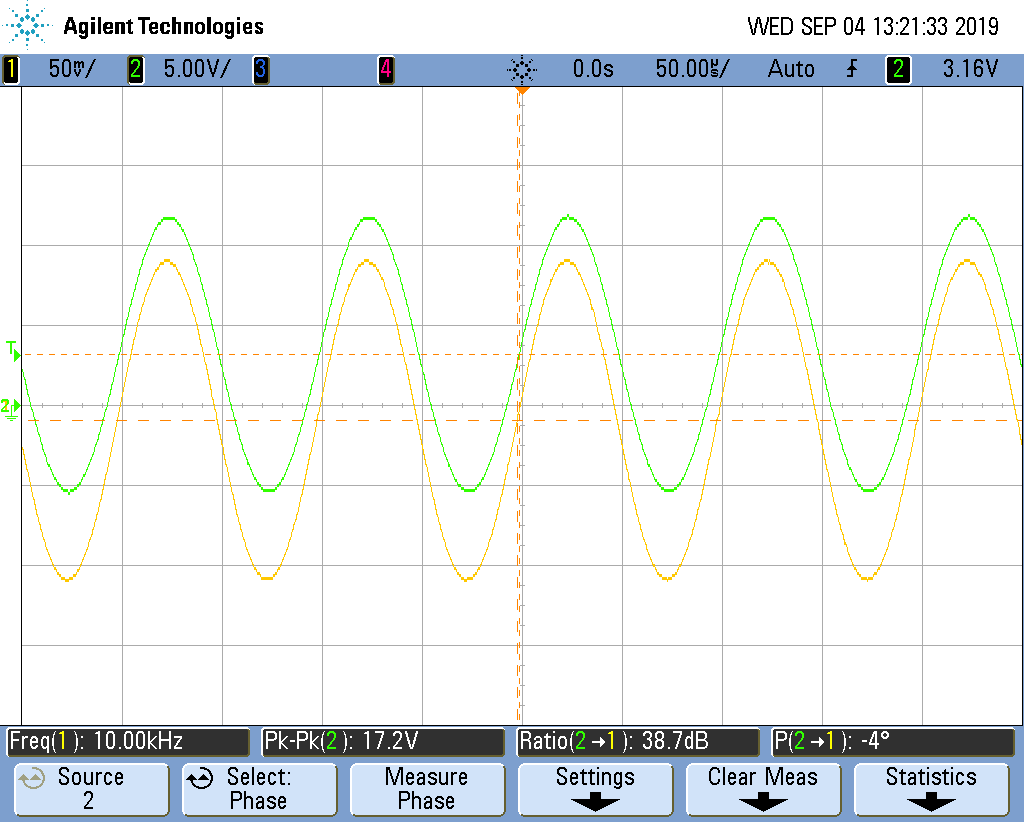
\includegraphics[height=10cm]{../Ex2/Informe/rsc/lm_0.png}
\caption{Medición de la tensión de salida a $10 kHz$ con el $LM833N$}
\label{fig:e2_lm_10k}
\end{center}
\end{figure}

\begin{figure}
\begin{center}
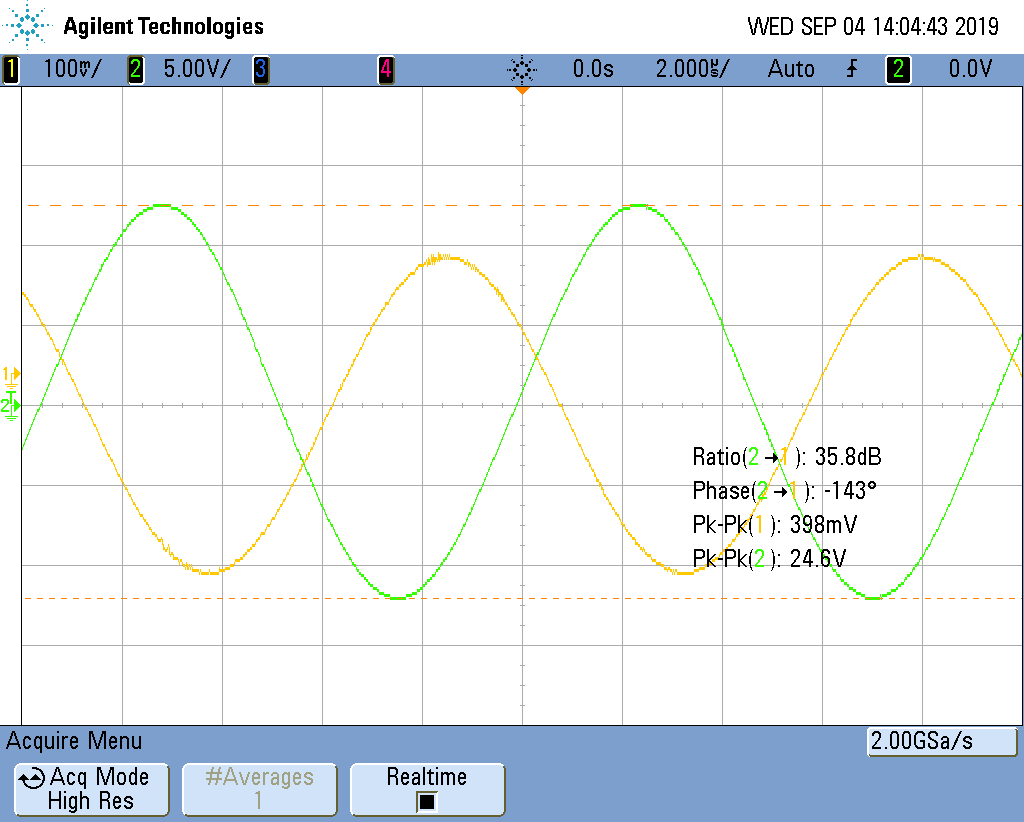
\includegraphics[height=10cm]{../Ex2/Informe/rsc/lm_1.png}
\caption{Medición de la transferencia en $f=106.5 kHz$ con el $LM833N$}
\label{fig:e2_lm_fB}
\end{center}
\end{figure}

\begin{figure}
\begin{center}
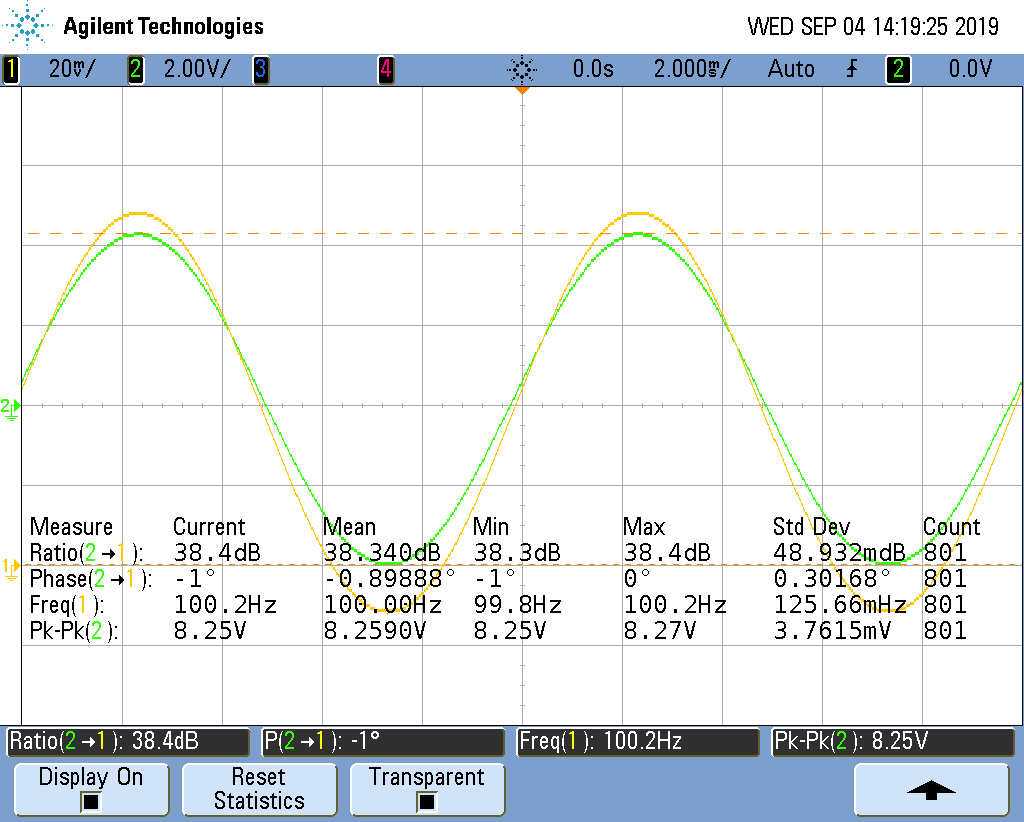
\includegraphics[height=10cm]{../Ex2/Informe/rsc/ne_0.png}
\caption{Medición de la tensión de salida a $10 kHz$ con el $NE5534P$}
\label{fig:e2_ne_10k}
\end{center}
\end{figure}

\begin{figure}
\begin{center}
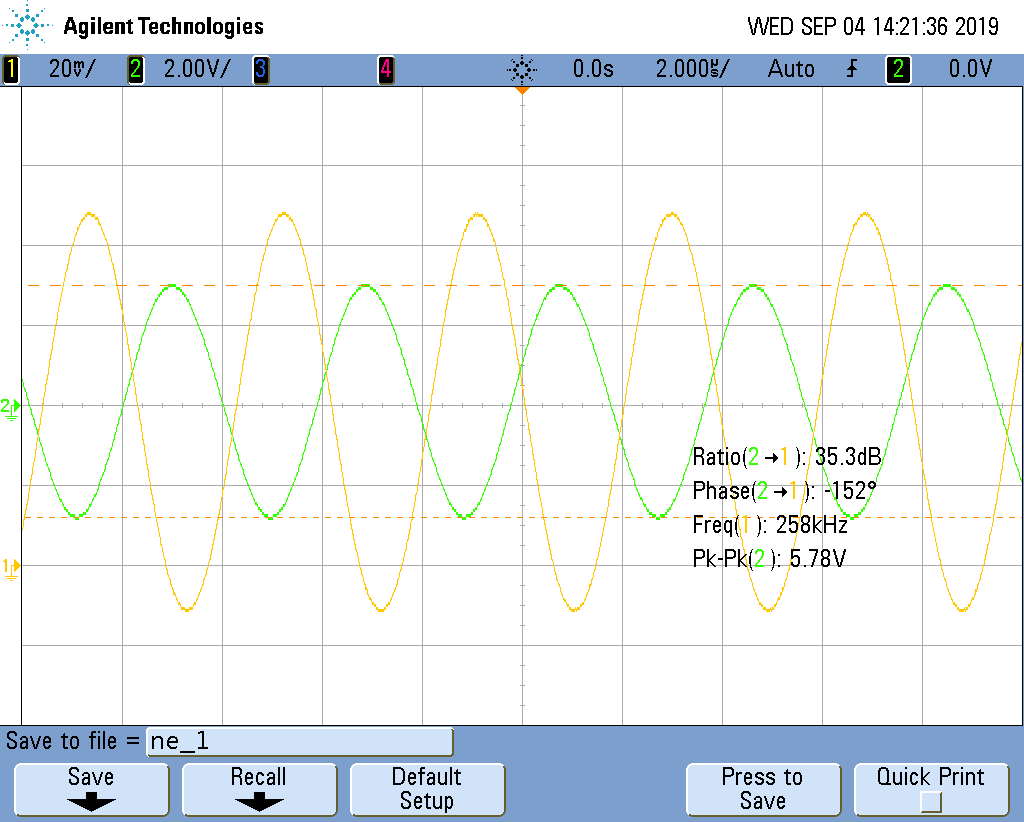
\includegraphics[height=10cm]{../Ex2/Informe/rsc/ne_1.png}
\caption{Medición de la transferencia en la frecuencia de corte con el $NE5534P$}
\label{fig:e2_ne_fB}
\end{center}
\end{figure}

\begin{figure}
\begin{center}
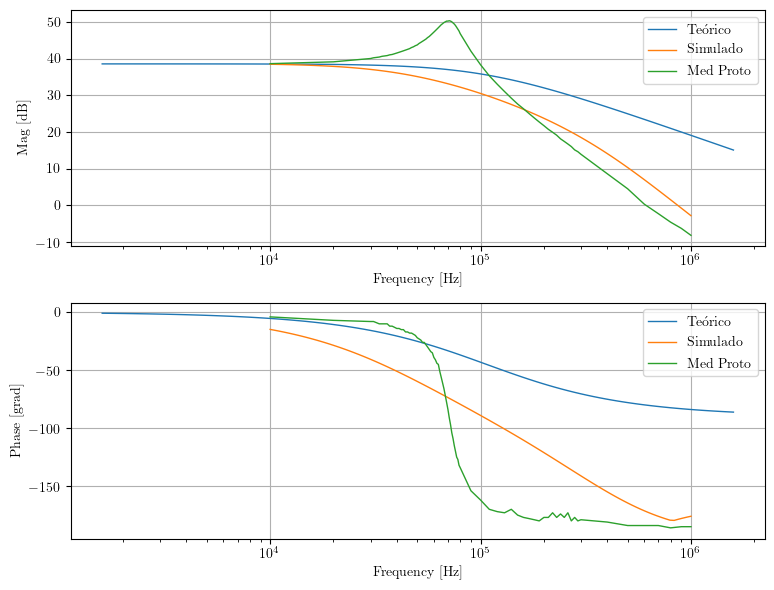
\includegraphics[height=10cm]{../Ex2/Informe/rsc/lm_bode_proto.png}
\caption{Respuestas en frecuencia del $LM883N$}
\label{fig:e2_lm_bode}
\end{center}
\end{figure}

\begin{figure}
\begin{center}
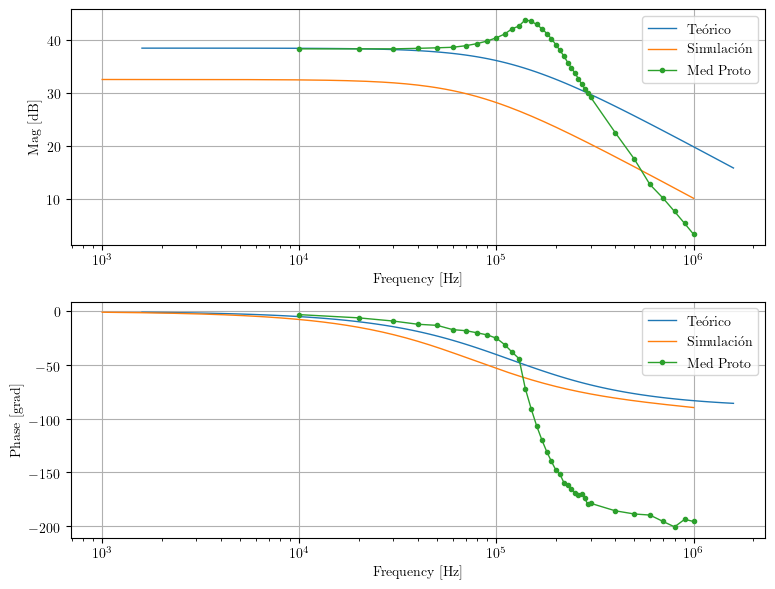
\includegraphics[height=10cm]{../Ex2/Informe/rsc/ne_bode_proto.png}
\caption{Respuestas en frecuencia del $NE5534P$}
\label{fig:e2_ne_bode}
\end{center}
\end{figure}

La primera diferencia observable en ambos circuitos es la presencia de un polo de segundo orden en las mediciones donde debería encontrarse un polo de primer orden, como indica el análisis teórico. Dado el sobrepico observado, se puede deducir que estos dos polos son complejos y conjugados.
Esto puede deberse a que dentro del operacional puede existir una capacitancia no contemplada en la hoja de datos, o la capacitancia inducida por las puntas del osciloscopio están agregando otro polo. Además, las capacitancias inducidas por el \textit{protoboard} también pueden estar afectando al circuito en general.

La presencia de este segundo polo es más apreciable en la respuesta en frecuencia de la fase cuando se utiliza el amplificador $NE534P$, la cual en la simulación y el modelo teórico desciende sólo hasta los $90^{\text{o}}$ en el rango de frecuencias medido.

La diferencia en la ganancia del circuito medido con la ganancia del circuito simulado se debe a que se utilizaron resistencias diferentes en ambos casos: en el primero una resistencia de $100k\Omega$ y en el segundo la resistencia de $220k\Omega$ indicada en la consigna. Esta diferencia en la magnitud de amplificación se debe a que existe una caída de tensión en $R_3$ comparable; por lo tanto el circuito amplifica una tensión menor a la ingresada, lo que es percibido como una ganancia total menor a la ideal.

Estas diferencias indican que hay elementos del modelo real que no se están contemplando en el análisis teórico ideal de los circuitos en cuestión.

\subsection{Impedancia de Entrada}
Se observa que la impedancia de Entrada del circuito decrece a medida que se aumenta la frecuencia.

\section{Conclusión}
Si bien los modelos teóricos y los modelos simulados sirven para predecir hasta cierto punto el comportamiento de un circuito amplificador, estos pueden llegar a no tener en cuenta o predecir cuestiones como el sobrepico encontrado en ambos casos de los circuitos.
Observando las distintas respuestas en frecuencias de ambos circuitos, se puede sugerir que si uno necesita utilizar un amplificador no inversor, aquel construido con un operacional $NE5534P$ conservará su nivel de amplificación en frecuencias más altas que el $LM833N$, peró deberá tener cuidado de utilizar resistencias que se aproximen a la resistencia de entrada del amplificador ya que puede tener una ganancia menor a la deseada si solo sela calcula con el modelo ideal.
Por otro lado, deberá tener en cuenta que el sobrepico presentado por el circuito construido con el $NE5543P$ alcanza una ganancia menor a la del construido con el $LM833N$, reduciendo el riesgo de quemar otras partes de la aplicación de este circuito.

\begin{figure}[h]
\begin{center}
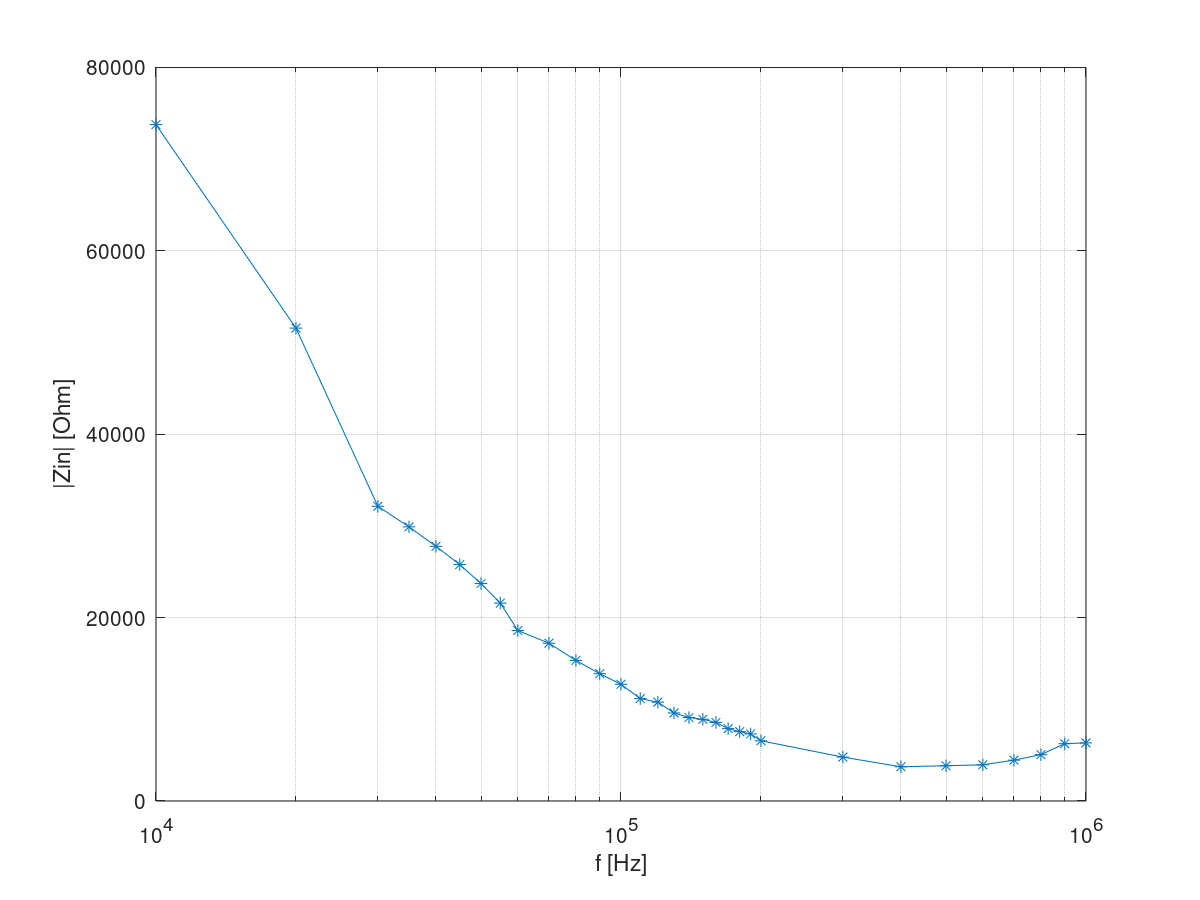
\includegraphics[height=6cm]{../Ex2/Informe/rsc/lm_proto_zin.png}
\caption{Impedancia de entrada del $LM833N$}
\label{fig:e2_lm_proto_zin}
\end{center}
\end{figure}

\begin{figure}[h]
\begin{center}
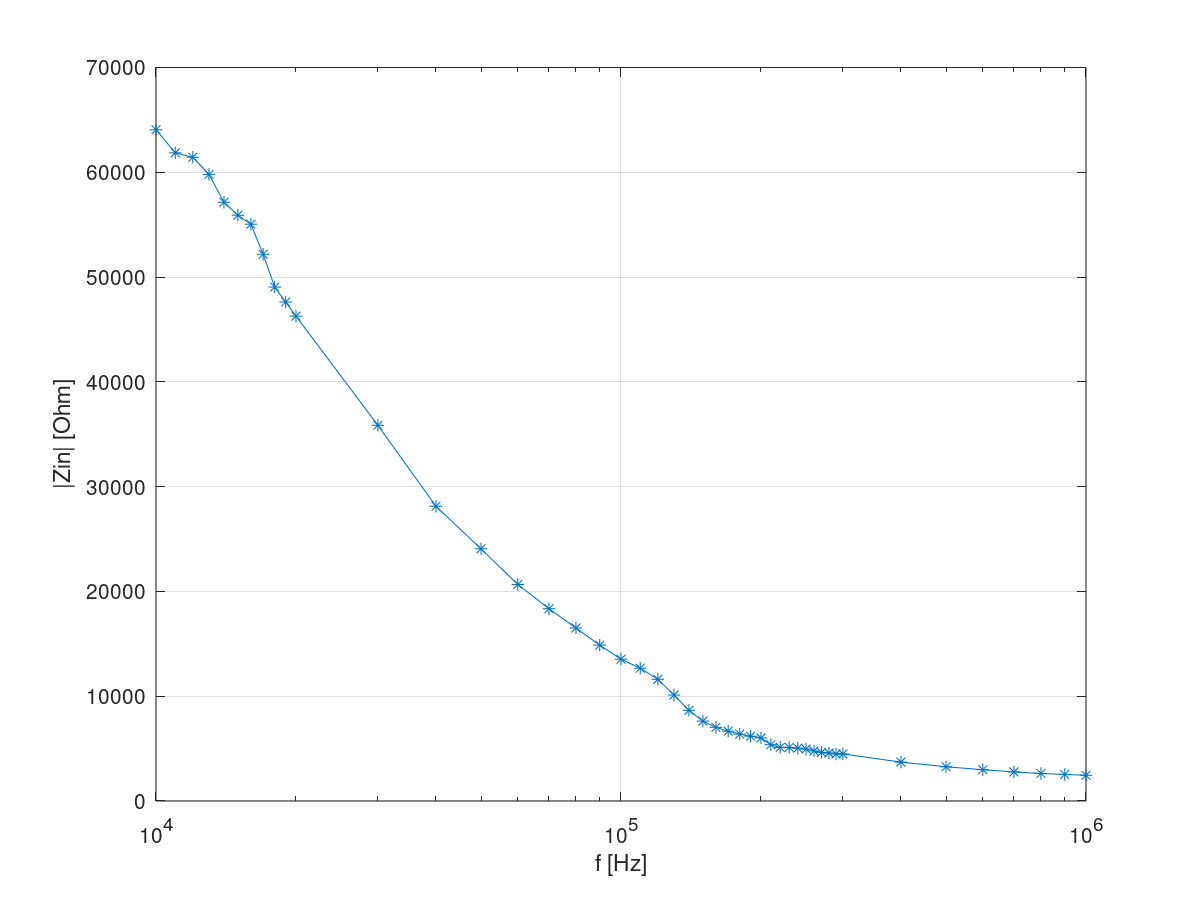
\includegraphics[height=6cm]{../Ex2/Informe/rsc/ne_proto_zin.png}
\caption{Impedancia de entrada del $NE5534P$}
\label{fig:e2_ne_proto_zin}
\end{center}
\end{figure}